\documentclass[12pt,fleqn,leqno,letterpaper]{article}
\usepackage{graphicx}
\graphicspath{{../figures/}}

\title{Luminosity}
\author{Cameron, M. \and Rosales, V. \and Westermann, J.P.}

\date{July 30, 2017}

\begin{document}

\maketitle
\newpage
\tableofcontents
\listoffigures
\listoftables

\newpage

Notes (Please Read):
\begin{itemize}
  \item print(df.to\_latex()) will give a latex export of the dataframe in the jupyter notebook, you can use this to quickly copy paste into latex
  \item plt.savefig(<path>) will allow you to save your figure as a png so it can be used in the document/presentation
  \item Make sure to commit and pull as much as possible to avoid merge errors
  \item Don't edit the styles of this document yet, will do that at the end
\end{itemize}

\begin{section}{Introduction}
  \begin{subsection}{Summary}
    TODO Will do this last
  \end{subsection}
  \begin{subsection}{Literature Review}
    \begin{subsubsection}{Luminosity-based Approach}
      TODO Michael: Try to accumulate as much as possible. We have such a long list of papers anyway.
    \end{subsubsection}
    \begin{subsubsection}{Natural Disaster Economics}
      TODO Viviana: obviously, as the expert.
    \end{subsubsection}
  \end{subsection}
\end{section}

\begin{section}{Data}
  \begin{subsection}{Data Description}
    TODO Micheal: Describe what the data looks like, how many observations there are, where we got it, who else has used it etc.
  \end{subsection}
  \begin{subsection}{Data Preprocessing}
    By the nature of the data, certain hurdles must be overcome before it's possible to model the luminosity data in any way. These issues include especially:
    \begin{description}
      \item[Volume]{While the number of observations is extremely low, as only annual images are available from 1992 to 2013, the dimensionality of each observation (image) is considerable. With a size of $16801$ by $43201$, every image contains $725820001$ pixels in total, which results in more than 700MB of disk-space required for only one image in uncompressed format. This also means that computations on the entire dataset are not possible with common personal computing architecture.}
      \item[Noise]{The data is inherently noisy and contains measurement irregularities stemming from e.g.\ human activity, orbital body positioning, luminosity radiance etc.\ Although the images have been corrected for solar and lunar influence, a look at the chart still suggests some noise level that differs}
    \end{description}
    \begin{subsubsection}{QGIS}
      TODO Viviana
    \end{subsubsection}
    \begin{subsubsection}{Python Architecture}
      TODO Jonas
    \end{subsubsection}
    \begin{subsubsection}{Denoising}
    \end{subsubsection}
  \end{subsection}
\end{section}

\begin{section}{Modelling}
  \begin{subsection}{Disaster Impact Models}
    Exploratory analysis and some basic models are a first step to assessing the impact of natural disasters on the luminosity time series. For this, we need to make a modelling decision regarding how the disaster (represented only as a single point location) can be geospatially associated with pixel luminosity values. TODO Jonas, literature on this?
    \begin{subsubsection}{Linear Distance-based Modelling}
      One practical mathematical choice is a function decaying with distance affecting areas or even individual pixels on the grid. The advantage of this method is that it is simple to explain, easily tuneable and leaves a lot of flexibility for modelling. Additionally, it captures the notion that areas in the vicinity of a disaster event are more likely to be affected than those further away by default.
      To trial this approach, we extracted 150x150 squares from the satellite image of the entire planet in a similar fashion as a convolutional neural network would apply to an image. Then we filter the top $t\%$ most luminous 'subimages', as we can generally disregard those parts of the world that contain no lights (oceans, deserts, etc.) and calculate 
      However, this approach makes some strong assumptions about the nature of natural disasters that don't hold in reality. An important factor in how much impact a disaster has on a region are geographical features: An earthquake will affect different areas differently based on their rockbed and geological consistency while e.g.\ storms and floods depend strongly on the topography. Nevertheless, the calculation of such a disaster coefficient yields promising results.
      \begin{figure}
        \centering
        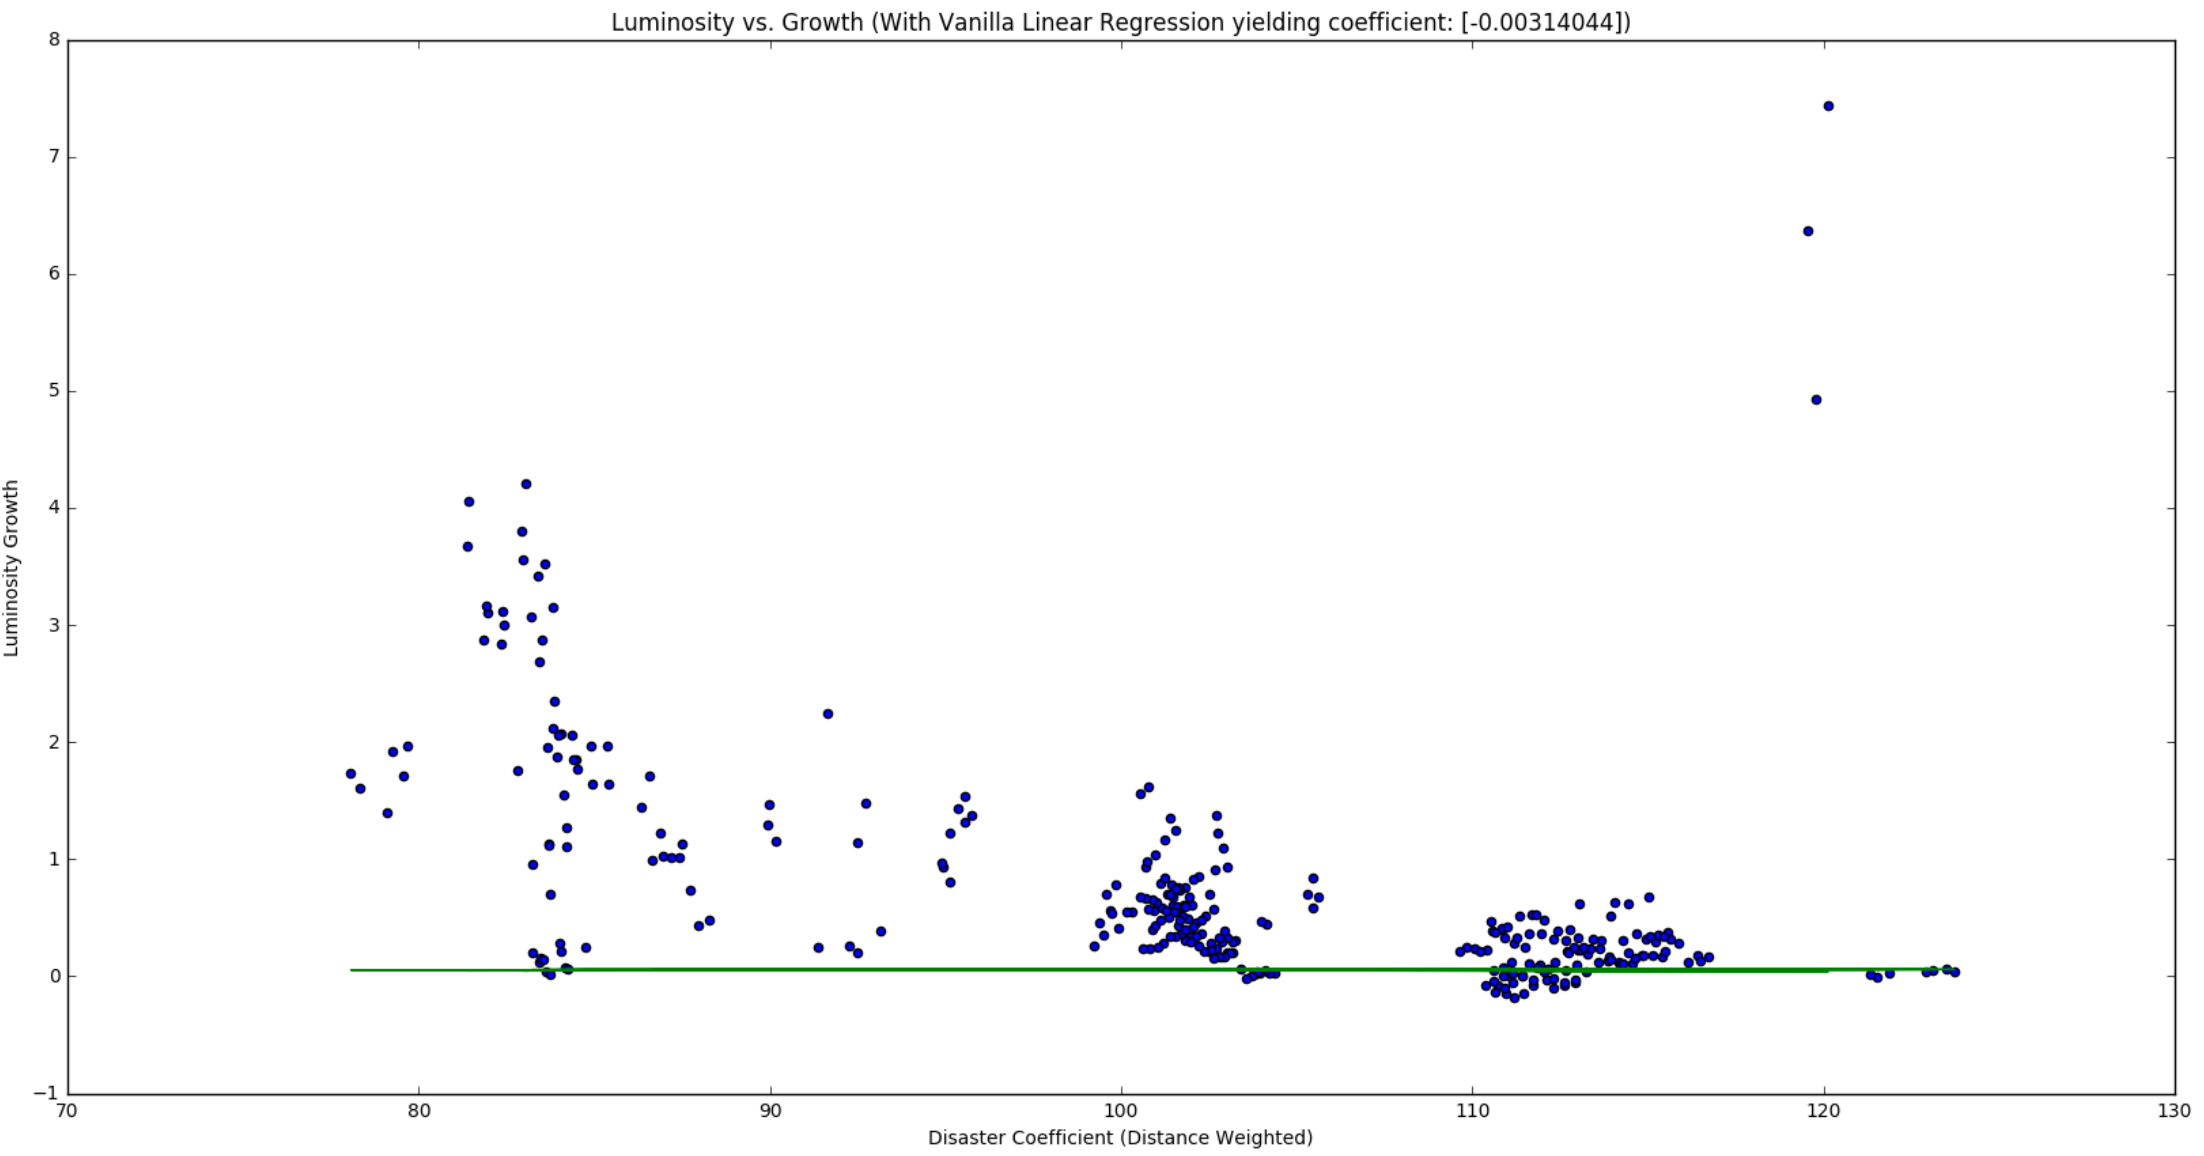
\includegraphics[width=1\linewidth]{linear-model-1}\label{fig:linear-model-1} %TODO: Adjust plot pngs to have sensible size for document
        \caption{Luminosity Growth 1992-2013 plotted against a linearly decaying disaster coefficient for 150x150 image sections.}
      \end{figure}
    \end{subsubsection}
    \begin{figure}[t!]
      \centering
      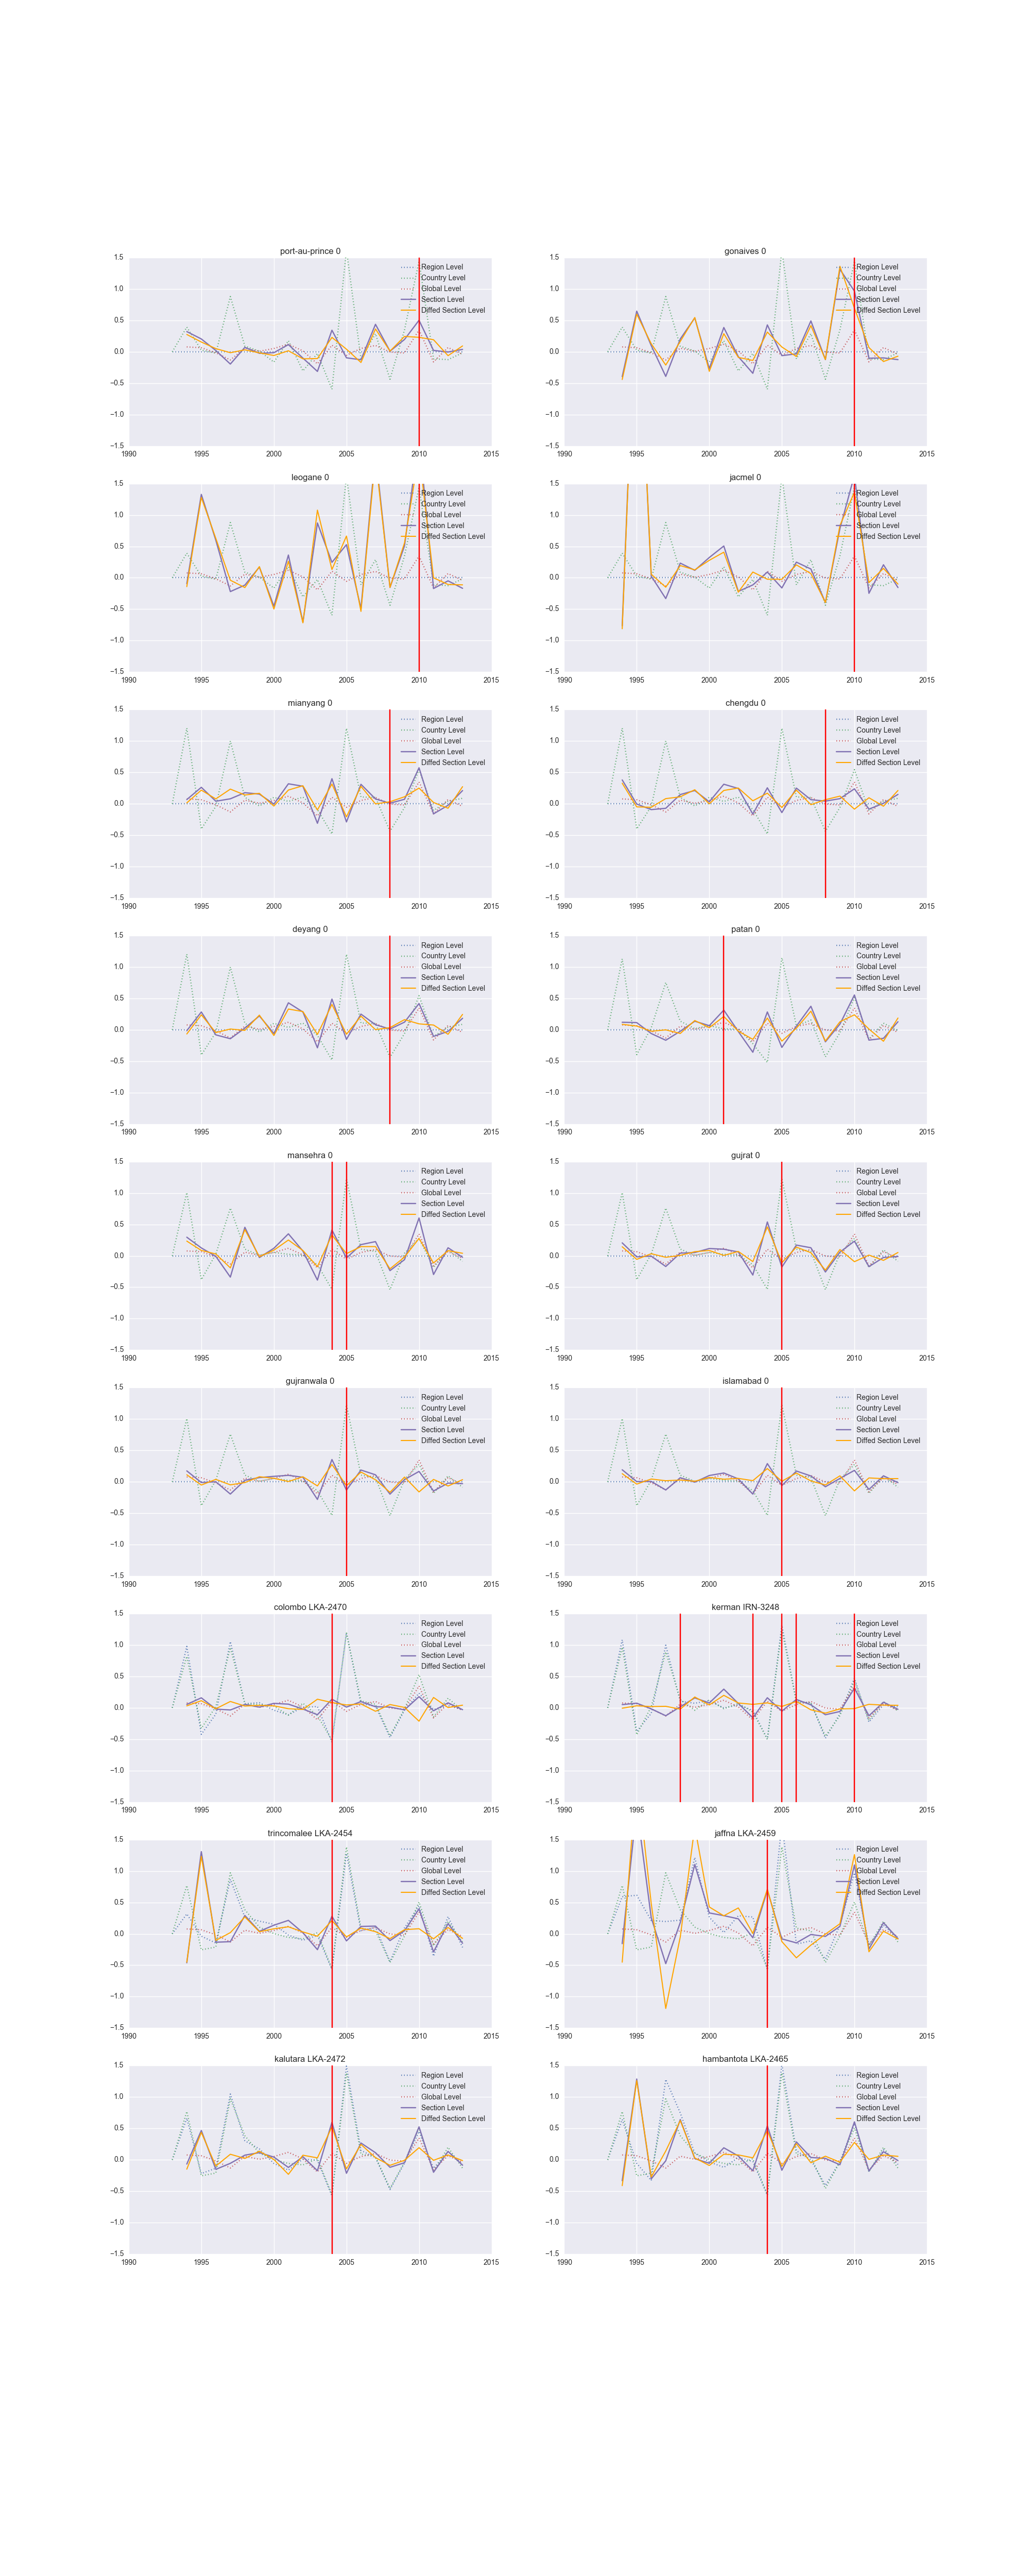
\includegraphics[width=1\linewidth]{pca_balancer_diffs}\label{fig:weighted_balanced_luminosity_sum_series} %TODO: Adjust plot pngs to have sensible size for document
      \caption{Luminosity Series Balanced by PCA Components}
    \end{figure}
    \begin{figure}[t!]
      \centering
      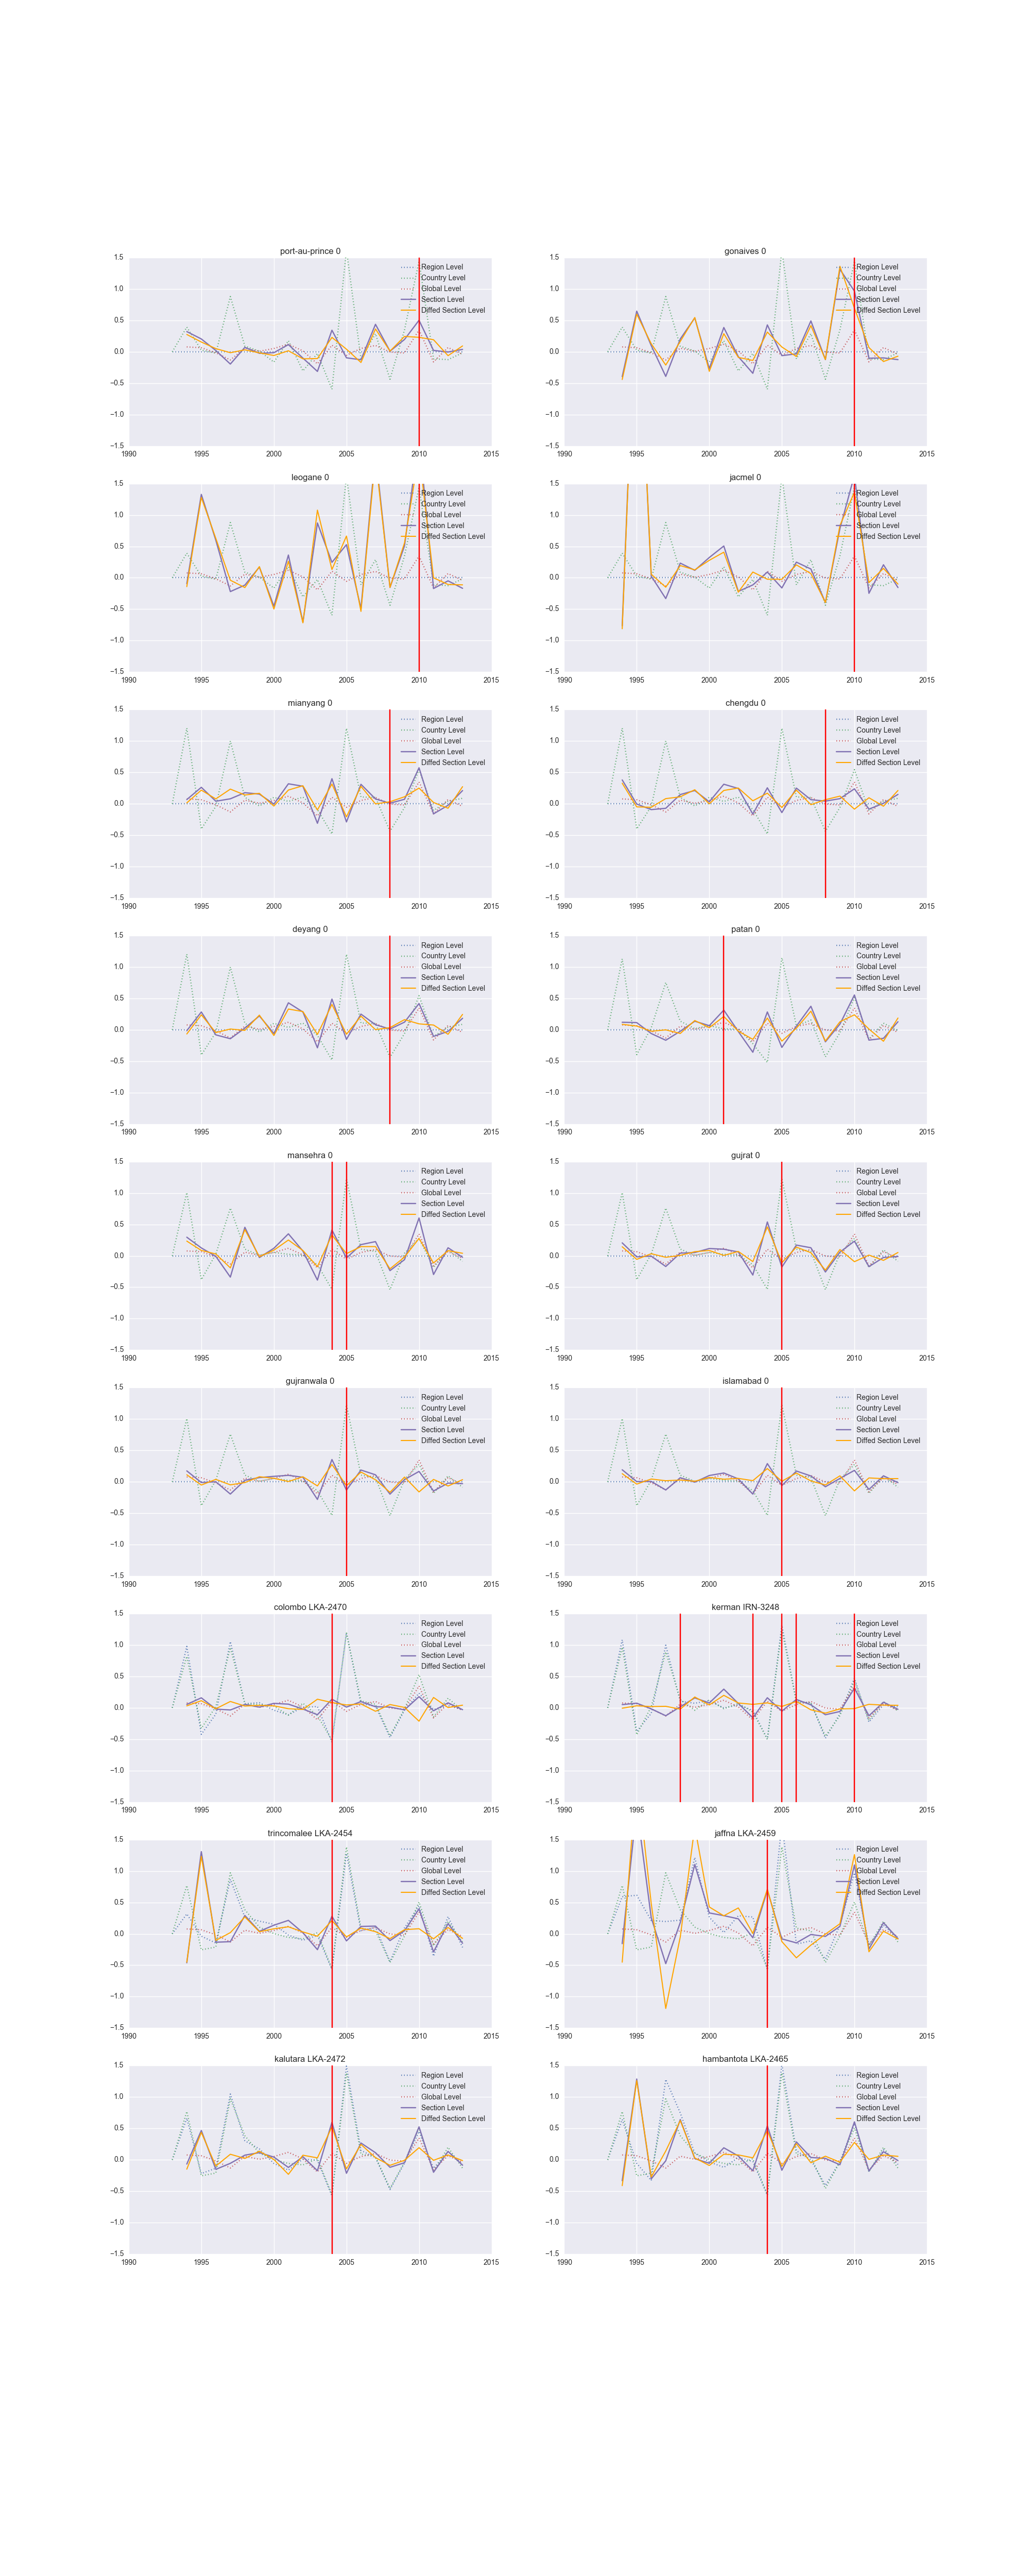
\includegraphics[width=1\linewidth]{pca_balancer_diffs}\label{fig:pca_balanced_luminosity_sum_series} %TODO: Adjust plot pngs to have sensible size for document
      \caption{Luminosity Series Balanced by PCA Components}
    \end{figure}
  \end{subsection}
  \begin{subsection}{Panel Model}
    \begin{subsubsection}{Region-based Panel}
      TODO Viviana
    \end{subsubsection}
    \begin{subsubsection}{Section-based Panel}
      TODO Jonas
    \end{subsubsection}
    \begin{subsubsection}{Dynamic Panel}
      TODO Viviana: Describe here how the model that you are using is constructed, where you got it, etc.
    \end{subsubsection}
  \end{subsection}
\end{section}

\begin{section}{Results}
  \begin{subsection}{Case Analysis}
    TODO Micheal: This is where your case analysis for different places goes, try to add some statistical tests etc.\ if possible. E.g.\ distribution of light one year vs the next compared to overall time series distribution changes (shocks).
  \end{subsection}
  \begin{subsection}{Modelling Results}
    TODO Viviana: Describe the results of the regression here, significant values and what those values mean.
  \end{subsection}
  \begin{subsection}{Conclusions}
    TODO Will do this just before the summary
  \end{subsection}
  \begin{subsection}{Outlook}
    TODO Jonas
  \end{subsection}
\end{section}

% -- Bibliography (APA style)
\bibliography{references}

\end{document}
